\documentclass[bibtotocnumbered, headsepline,normalheadings,12pt]{report}
\usepackage[utf8x]{inputenc}
\usepackage{ulem}
\usepackage{color}
\usepackage[polutonikogreek,english]{babel}
\usepackage{ucs}
\usepackage{booktabs}
\usepackage{setspace}
\doublespacing
\usepackage{multirow}
\usepackage{listings}
\lstset{basicstyle=\footnotesize\ttfamily,breaklines=true,showstringspaces=false,numbers=left,frame=single,prebreak=\mbox{$\hookleftarrow$}}
\usepackage[hidelinks]{hyperref}
\usepackage[a4paper,margin=2cm]{geometry} 
\usepackage{scrpage}
\usepackage{alltt}
\usepackage{float}
\usepackage{graphicx}
\definecolor{darkblue}{rgb}{0,0,.5}
\hypersetup{pdftex=true, colorlinks=false, breaklinks=true, citecolor=darkblue, linkcolor=darkblue, menucolor=darkblue, pagecolor=darkblue, urlcolor=darkblue,
pdftitle={CACGD 2011 Practical Excercise Report},
pdfauthor={Bartholomäus Dedersen},
bookmarks=true,
bookmarksnumbered=true,
bookmarksopen=true,
bookmarksopenlevel=2}
\usepackage{tabularx}
\pagestyle{headings}
\newcommand{\gdir}%
   {\foreignlanguage{polutonikogreek}}
\usepackage{color}
 \definecolor{light-gray}{gray}{0.80}
\newcommand{\CS}{C\nolinebreak\hspace{-.05em}\raisebox{.6ex}{\scriptsize\bf \#}}

\begin{document}



\begin{titlepage}
\thispagestyle{empty}
 \begin{center}
 \begin{figure}[htbp]
    \centering
     
\includegraphics[width=0.75\textwidth]{fhkiel.png} 
\end{figure}

  \vspace*{2.5cm}
 {\bf \huge CACGD 2011 Practical Exercise Report}
 \vspace*{1cm} \\
 {\Large Game Development\\}
 \vspace{0.5cm}
 {\Large \bfseries Bartholomäus Dedersen\\}
 \vfill
  \vspace*{1.5cm}
\begin{table}[h]
    \centering
    \begin{tabular}{l l}
        Date of Excursion: & Summer 2011 \\ 
        Place: & Iraklion, Crete, Greece \\ 
        Course: & Information Technology \\
        %Date: & 3.1.2013\\
        Date: & \today\\
    \end{tabular}
\end{table}

 \end{center}
\end{titlepage}


\begin{abstract}

    In this report about the practical part of the ``Computational Aspects of Computer Games Development'' programme for two weeks in Crete a
    game programming with the Python programming language is described. The controller is a neural interface for brainwave wavelength reception 
    through three skin-applied electrodes. The game is themed after a fictional Cretan Zombie incursion after the actual event.

\end{abstract}

\tableofcontents \newpage


\chapter{Introduction}
\label{chap:intro}
\gdir{Μετα δέ την του βίου τελευτην ου  μετα ληθης ατιμοι κεῖνται, αλλα μετα μνημης τον αει ξρονον ὑμνοũνται.}\\
-- Xenophon
\vspace{15mm}

This written documentation is a part of the two week conference and tutored exercises in the Cretan state capital Iraklion. The host was the
Technical Educational Institute of Crete, a university with emphasis on applied technology. The conference preparation was done especially through the 
department of Computer Sciences, visible through the timetable.\footnote{Available at \url{https://cacgd2011.teicrete.gr/?q=content/program-lectures}.}.

The author of this work was part of the team from the German Fachhochschule Kiel and reported his personal experience in an formerly online available
diary. This report is supposed to contain the technical description of the proceeding practical lessen from the excursion. Worthwhile to mention 
members of the other college teams were not bound for such task as it functions as an addition to the regular curriculum of the event.
Skills learned should be applied in the resulting game or educational entertainment tool.

Other members of the authors team presented their own results, i.e. a location-based game and a helicopter simulation for children on a mobile platform.

The task was done without the acquired technique of proper software engineering. Instead, a more spontaneous and agile development process was
chosen due to the small team size and new field of work.

The author wants to express his gratitude for having the option to experience Greece and learn new ways of thinking. 

A preceding work from the author is recommended to read as it contains more information in regards to the neural interface, see~\cite{pm}.


\chapter{CACGD Programme}
\label{chap:cacgd}

``Computational Aspects of Computer Game Development'' is part of a series of academic exchanges. Every year until Crete, the 
two week programme was hosted by another European university. Students were housed in the college's respective dormitories and 
supplied with necessary food.

In 2011 on the 11 July, a Monday,  a wide range of educational institutes from Czech, Canada, Great Britain, French, Greece and Germany participated, mostly by
students from Bachelor's courses. The total amount of students was about 70. Half of the audience during the lectures was 
Greek as interested students were invited. Hard-working, responsible organisator from the Greeks George Papadourakis held a
welcome speech and presented the final lecture programme. His own presentation was scheduled at the last day of the 14-day programme.

Instead, George Mamakis held his presentation about ``Visual Perception in Graphic Design – Neuroaesthetics''. Generally spoken, the 
topic evolved about the perception of visual stimuli and how people process and judge them. Especially how feelings are associated 
with pictures. A practical part was the design of a paper sign, capable for using in demonstrations, about the economic crisis. The
authors group solution mainly consisted of a weight scale with weight emphasis money on one side while a house as a sign of material property on 
the other side.
The in-between canteen breaks with associated food description is part of the lost online diary and will not be elaborated in addition to the 
rather mediocre rating giving here.
Second part of the day was filled with George Triantafyllidis' ``The XNA environment for game development''. XNA is used for rapid prototyping of 
computer games and deployment on console based platforms as the XBox from Microsoft or regular Windows machines. It is very interwoven with the
underlaying Dotnet framework and centers around C\# for its main programming language. It has an in-build graphical engine with wrappers for 
Direct3D for acceleration. The idea for rapid development was taken from this lecture for the practical part of this report.

\begin{figure}[H]
    \centering
    
\includegraphics[width=0.6\textwidth]{xna.png}%
    \caption{XNA logo. Source: xblafans.com}
    \label{fig:xna}%
\end{figure}

The next day began with the first non-TEI lecturer Nadine Pasternak from University of La Rochelle in France. His topic, ``Cross-Cultural Communication and Computer Gaming'', was centered about the psychological value of computer games in means of understanding messages from non-native culture origins.
Concluded, gaming can be used to enhance the existing ways of communication between different people and games can be designed to be 
understandable by anyone. The principle of ``easy to learn, hard to master'' was also used on the practical game, similar to chess.

Michel Eboueya, another French lecturer from La Rochelle, presented different ways of graphics in computer games in his ``Computer Graphics In Games Design and For Games''. He showed the way clipping works, i.e. the removal of computational power from processing non-visible graphics to the player. Basics of 
3D design were demonstrated but the lecture was missing practical parts to try out the theory.

On Wednesday ways of ``Data Visualization'' from Nikos Vidakis, a member of the Medialab of the TEI, were shown. As an example figure~\ref{fig:opte}, shows
a simplified graph of various communicating subnets in the Internet. A number of human-selected top level domains are part of the image.
Another explained method were statistics as an educational and entertaining way of presenting game data. Graphs can even represent whole game 
series, e.g. Europa Universalis from Paradox Interactive. The figure~\ref{fig:eu} shows a great example by visualizing the numerical game data into
easier understandable pictures.


\begin{figure}[H]
    \centering
    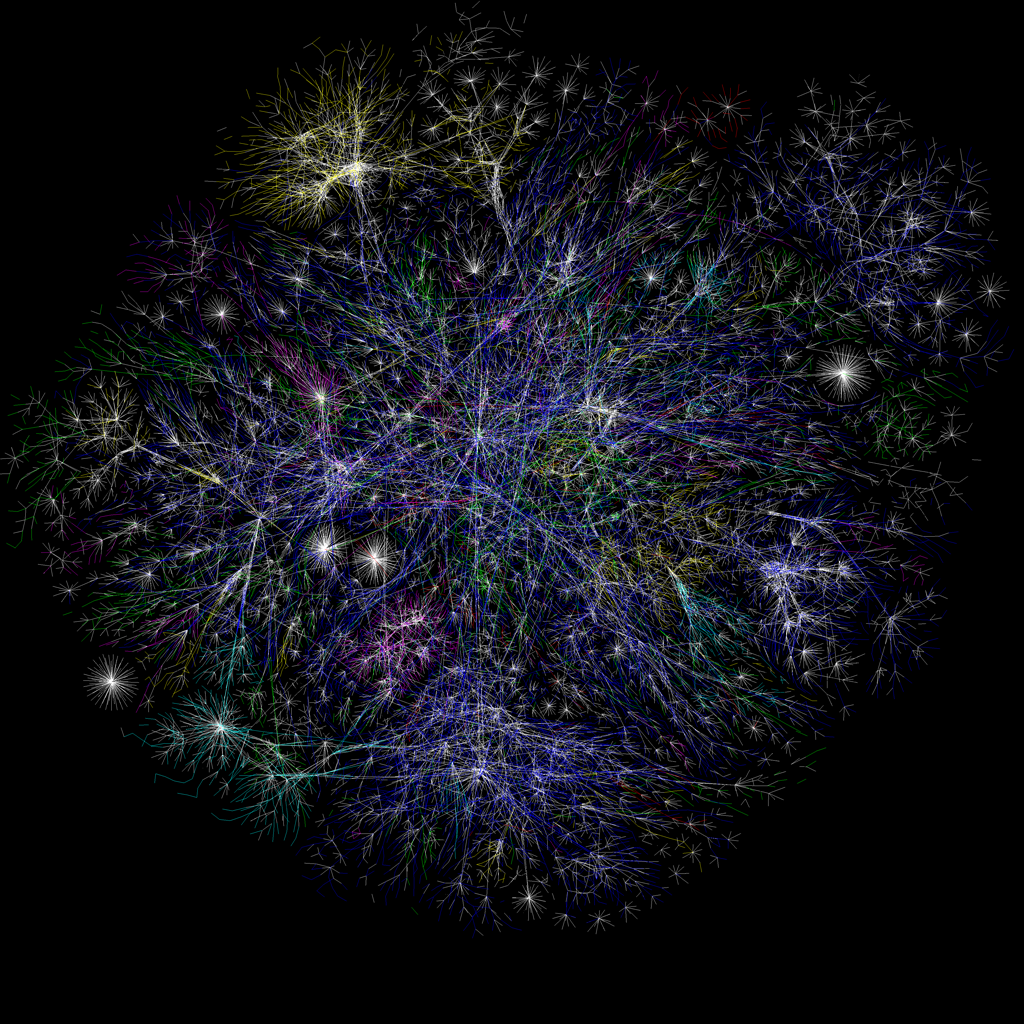
\includegraphics[width=0.6\textwidth]{opte.png}%
    \caption{Visualization of Internet Traffic in Subnets. Source: opte.org}
    \label{fig:opte}%
\end{figure}

\begin{figure}[H]
    \centering
    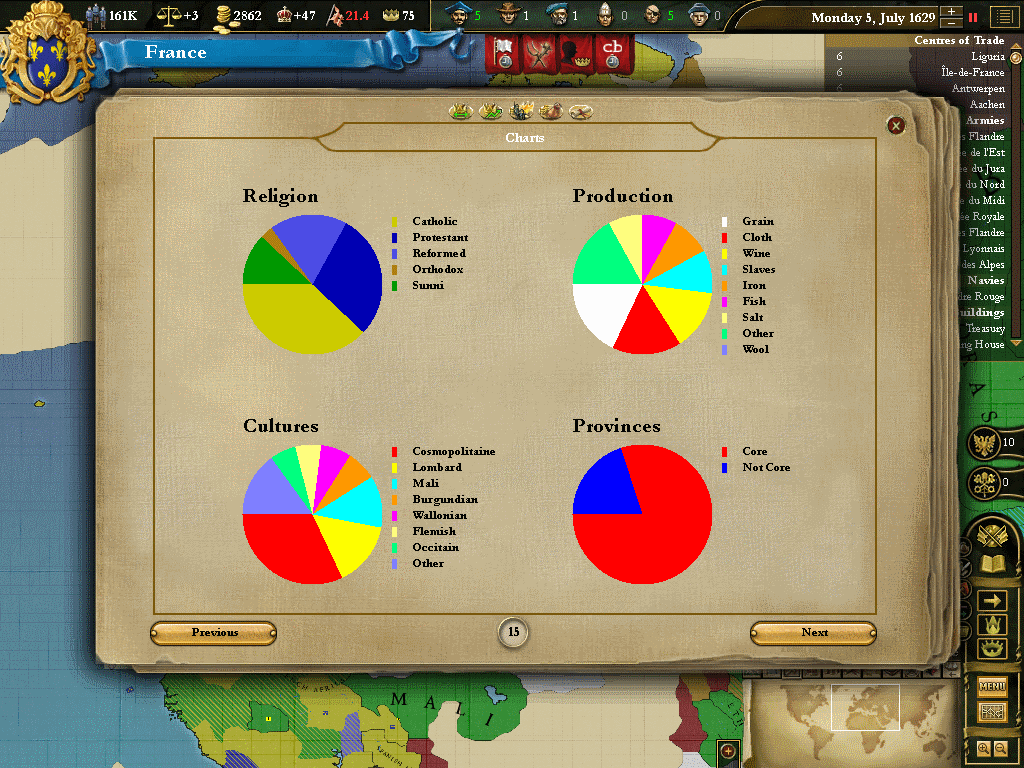
\includegraphics[width=0.6\textwidth]{eu.png}%
    \caption{Europa Universalis 3 as example for data-centric games. Source: paradoxplaza.com}
    \label{fig:eu}%
\end{figure}

After the lunch the highly anticipated ``Security Issues in Computer Games'' by TEI's Harry Manifavas showed the listeners how in-game payments are 
procured and how real money can be lost in such games. The economics of virtual currencies in games like Linden Dollars in Second Life are similar
to real-world currencies, including fluctuation and speculation. As an example, the worth of Bitcoins, the virtual and completely based in computing power,
not in trust, is shown in figure~\ref{fig:bc}. The total availability of bitcoins is limited by the total calculation of a specific hash function as further
explained in~\cite{bitcoin}. The ability to forge such transaction is limited to the extend the attacker can provide a higher amount of computation power 
compared to the whole distributed Bitcoin network.

\begin{figure}[H]
    \centering
    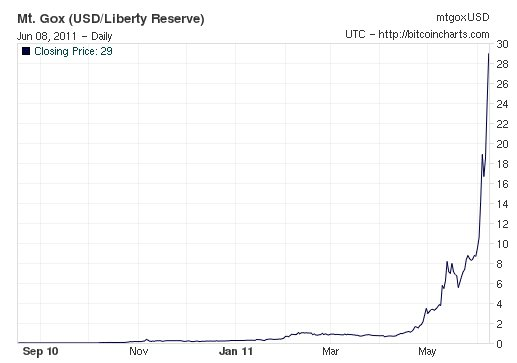
\includegraphics[width=0.6\textwidth]{bc.jpg}%
    \caption{Bitcoin to USD exchange rates. Source: bitcoincharts.com}
    \label{fig:bc}%
\end{figure}

Thursday was the day of neuronal networks and artificial intelligence. In the morning, Ali Ghorbani from the University of New Brunswick in Canada was 
giving a speech about ``Unsupervised Learning''. He gave a firm introduction to artificial learning with Hebbian networks as to

\[ w_{ij} = \frac{1}{p} \sum_{k=1}^p x_i^k x_j^k\]

where the connection between the neurons \(x_i\) and \(x_j\) is used to calculate the weight \( w \). It goes summed over generations called \( k \) in \( p \) 
training patterns. The formula simulates the learning in the simplified weight value for finding patterns in large input datasets. Similar learning is 
applied in the practical exercise in addition to a factor which weights the different wavelengths according to their physical reaction.
The opposite of supervised learning where a target value is precalculated or given by a human so the weights can be adjusted.


In the afternoon, Claude Frasson from the University of Montral in Canada had a talk
about ``Intelligent Tutoring Systems''. The topic evolved around educational systems for teaching support. Mainly projects for highschool teaching 
were shown.

The last day of the week was introduced by the British archeologist Gareth Owens. His talk about his DVD project about Cretan ancient history 
was dominated by his enthusiasm for the Phaistos disk. The multimedia effects of the DVD have video snippets combined with interactive moving sprites, 
simulating an excavation. Sound effects encapsulate the educational content in a game-like immersion. Practical part of the lesson was a discussion about
the possible meaning of the yet unknown content of the writing on the disk as shown in figure~\ref{fig:pha}. The vocal intonation is known but the 
meaning of the context and even words of the used language Linear A. The current hypothesis of Gareth Owens concerning the face symbol with 
spiked hair is the connected with the meaning of ``mother''.


\begin{figure}[H]
    \centering
    
\includegraphics[width=0.8\textwidth]{pha.png}%
    \caption{Front of the Phaistos Disk. Source: couk.com}
    \label{fig:pha}%
\end{figure}

The afternoon lecture was also held by Mr Owens and were focused around the Minoan history of Crete. Strabo writes about Crete that it ``flourished from the 
excellence of the soil, which is peculiarly adapted for breeding horses, and the growth of fine crops.'' in his \gdir{Γεωγραφικά}. Minoans lived 
before him on the island from roughly 2500 to 1500 BC and represented native inhabitants of Greece, so called Pelasgians. Strabo says ``that the Pelasgians had been a great people can be documented also by other sources. Namely, Menecratos Elaita, tells us in his book about the origins of the cities that the entire maritime region which now is called Ionia, starting from Mycale and the neighboring islands, has formed once the dwellings of the Pelasgians.''

First appearance of agriculture in Europe coming from the Middle East is linked to Crete as well as the mythological tale of the Minotaurus. Moreover, 
a relation to the Argonauts which searched for the Golden Fleece under the hero Jason could be established as ancient Crete was a hub for trading and 
was renowned with its riches in gold. Their ship, the Argo, is supposed to be buried on Crete.

Basic mythology was needed as the weekend's excursion lead the students to the archeological site of Knossos. It was the ancient ruling palace of the Minoan
king with a combined grain storage. The food was collected by the king and guarded for asserting power over the peasants and secure emergency ratios for 
upcoming droughts. Sophisticated inventions as a non-electric climatization were found on the excavation site. Cold air from the sun overcast hill towards
the coast went through internal wind canals to the top floors of the palace.

``Survey on Game AI theory and Algorithms'' on the next week's Monday was held by George Mamakis were the link was explained to his first lecture about
the effects of graphics. Students were animated to develop their own game formulas. George Bebis from the University of Nevada in USA showed medical 
usage of computer vision and showed his research lab with a short introduction to his scientific area. Image processing is also used in games for collision 
detection. Moreover, prototyped hardware for automatic traffic measurement of was shown.

\begin{figure}[H]
    \centering
    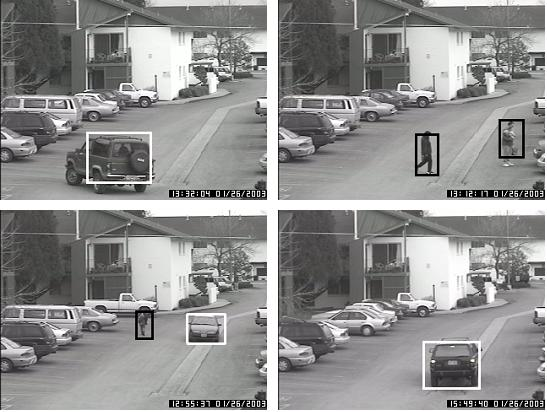
\includegraphics[width=0.8\textwidth]{bebis.jpg}%
    \caption{Traffic Detection and Analysis. Source: cse.unr.edu}
    \label{fig:bebis}%
\end{figure}

Next day's morning started with a lecture about game ethics by the British lecturer Paul Javis from the University of Glamorgan. Problematic questions as 
how to depict gore and violence and other questionable but realistic content is shown by example in games. The students were split in different groups which 
had to prepare and present arguments of one side for a specific question. Later on, the results were presented in a talkshow-like discussion with two 
groups arguing and the other students watching and judging about the \textsl{ethically right} position. As Zombies are ethically accepted when the 
violence level is kept under a certain culturally dependent threshold which is aimed for in the practical part only a minor part could be used.

``Principles of Artificial Intelligence'' from Andrew Ware from the same university as the previous speaker gave a general introduction to artificial learning 
and tried to show examples of Non-Player character behaviour in current games. The limitations of a complete simulation in regards to computational resources
were explained in a slide show.
Wednesday continued the speaks of the previous days.

Michal Hradiš from Brno University of Czech Republic introduced new methods for interaction in games in his talk. The author of this work got his 
inspiration by the man-machine interface from this lecturer. 3D glasses and other gear was also part of Thursday's morning.

\begin{figure}[H]
    \centering
    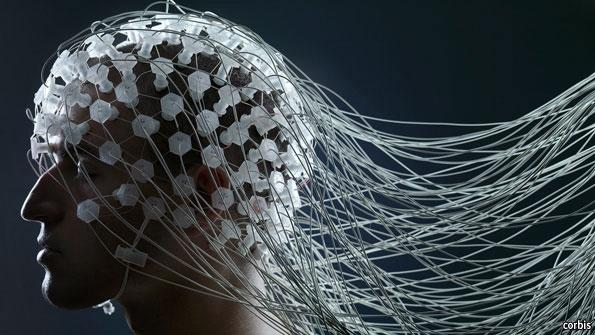
\includegraphics[width=0.6\textwidth]{eeg.png}%
    \caption{Futuristic EEG Device. Source: digitaltrends.com}
    \label{fig:bebis}%
\end{figure}

The second half of the day was succeeded by the same lecturer where he presented more real-world practical smart home implementations of entertainment. 
Augmented reality as an addition to the typical game experience was discussed and how such devices could alter the communication structure of the society.

On the last day of the games programme Helmut Dispert\footnote{Supposedly one, if not the only, reader of this document.} gave an overview of 
Ambient Intelligence. The author of this work wrote numerous exams and reports about this topic and was the main \xout{claquer} critique listener.  
The topic was a general introduction to the idea of ubiquitous computing, available devices on the market and location based services.

George Papadourakis held the final presentation about Quake 3 and general first person shooters. Mainly, the final certificates were handed out 
with a special souvenir from Crete.

\begin{figure}[H]
    \centering
    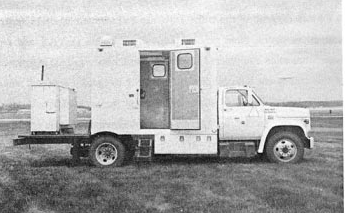
\includegraphics[width=0.5\textwidth]{earlynode.png}%
    \caption{Early Mobile Node. Source:~\cite{Chong}}
    \label{fig:node}%
\end{figure}


\chapter{Game Idea}
\label{chap:idea}

Starting a game is usually combined with the creation of concept art and background stories. The process is defined by the size of 
the final game and its intended audience. Technical prerequisites should be defined and specified and alternatives to requirements 
analysed.
As the game is developed solely by the author and has a specific requirement of a brainwave scanner the planning parts of the 
game are kept to the required minimal setup.

The background story is a fictional zombie incursion on the island of Crete. An unsuspecting student of the TEI finds a clay item
similar to the Phaistos disc while on vacation in Rethymno. The mysterious ruins as depicted in~\ref{fig:ret} of the old town open imagination to many uses
in previous times. Its last use was a fortress but the foundation and prominent place in the landscape suggest older uses.

\begin{figure}[H]
    \centering
    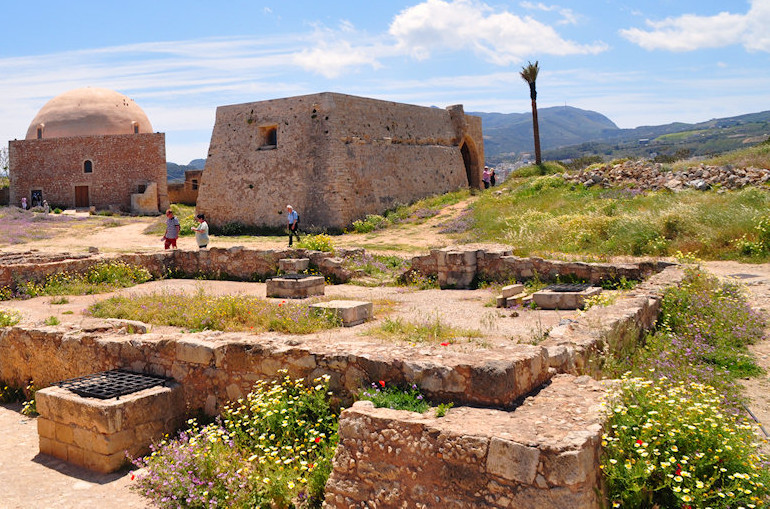
\includegraphics[width=0.6\textwidth]{ret.jpg}%
    \caption{Rethymno Ruins. Source: grieksegids.info}
    \label{fig:ret}%
\end{figure}

Unknowingly, the student's action released a hidden curse from the ancient ruins. An unknown king from the past ordered the creation of this 
last remnant for the protection against grave robbers. He could not decipher the ancient text on the disc, warning him of the effects of the curse.
His failure resulted in a insatiable hunger for knowledge, more directly, for brains. He was turned into a Zombie.

His aim is the collection of brain images, called sprites, but as the player is a Zombie he cannot use direct action. Only through his remaining will,
i.e. the brainwaves, he can steer himself for calming his hunger.

The time separation for an in-game action is defined by a specified time needed for the player to gain or loose concentration. One idea was to 
keep the time with a on-screen countdown but the mere visibility of a clock altered the game's result to a monotonous output. Ideally, another 
player is required to decide the time for committing the walking action towards the aim, i.e. the brain.
For comparison a high-score counter is shown on the screen in addition to visual representation of the current status of the brain's emitted waves. 
An acoustic signal shows the player if an object is hit.
The acting player's in-game representation of a Zombie moves with acceleration, giving the difficulty of the game which consists of a 
left or right vector and the initial power for the movement of the main sprite.

Main aim of the game is to train the main player's ability to concentrate and relax on will. Experimental users reported a similarity to 
meditation as techniques as Yoga contain elements of tension and release. 

Other similar games include popular mobile platform games like ``Plants vs Zombies'' or ``Angry Birds'' while the interface part can be only found on
experimental setups.

\begin{figure}[H]
    \centering
    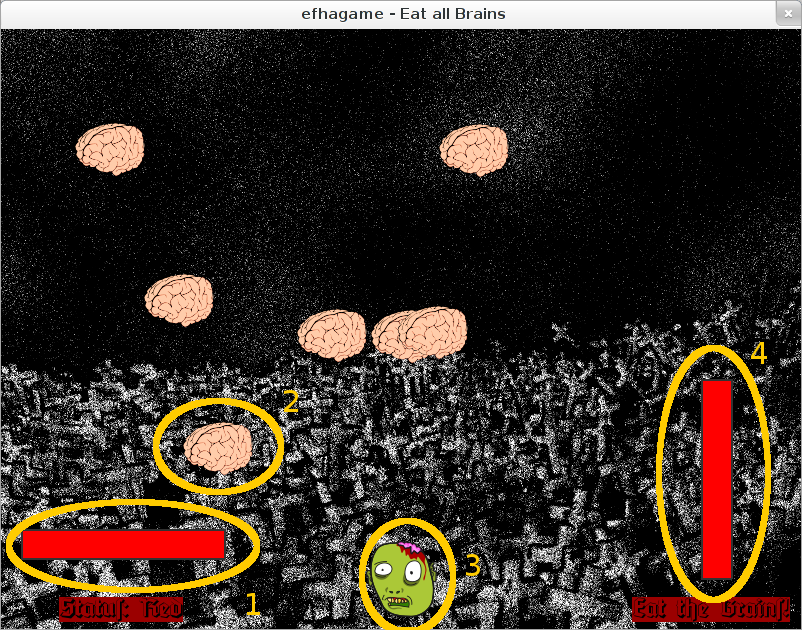
\includegraphics[width=0.8\textwidth]{game.png}%
    \caption{Screenshot of Main Game}
    \label{fig:screenshot}%
\end{figure}

Figure~\ref{fig:screenshot} shows the layout of the game elements in an actual screenshot.

\begin{enumerate}
\item Vertical designation indicator going from 0 to 180 degree from the bottom line of the game window.
\item Collectable brain sprites will spawn in the screen to collect. Multiple items can be gathered with one player movement.
\item Main game avatar at an lightly elevated position from screen bottom.
\item Movement strength for the next shot.
\end{enumerate}

The background is from a computer generated image from a free database with many filters for the unobtrusive design. It is fitted for the
Zombie theme as they are often shown combined in popular culture.

First prototyped versions of the game as visible in the development history of the distributed development version control Git had various placeholder graphics
until they were designed by the author's long term supplier of academic paintings. The screenshot shows the most current and final version.

As an entertaining and immersive element the player avatar moved with friction:

\[ F_\mathrm{f} \leq \mu F_\mathrm{n} \]

where \( F_\mathrm{f} \) equals the resulting speed from applied friction on the original static movement speed \( F_\mathrm{n} \) from the 
friction coefficient  \( \mu \). This factor is variable between the acceleration time until the main sprite reaches its furthermost position after
one movement and the swinging-back at the end. The final movement resembles the feeling of having the player's avatar strung up on a rubber band. The
friction is about 15\% higher in the last stage. 
The effect on the player should be a more elastic feeling of the game in contrast to a static and preemptive movement. It can be compared to the
object-throwing mechanism of ``Angry Birds'' where the bird flies with a ballistic angle towards its target.

Another big part of the game idea is the planning and development of the interface part. Both indicators, vertical alignment and movement speed, are
derived from the main player's cumulated brain waves over a period of time. The part is available at~\cite[p. 11--28]{pm}.

Noteworthy, the description of the used neural network and its underlying idea and theory can be found at~\cite[p. 4--8]{pm}.

\chapter{Framework}
\label{chap:framework}

The game and its required modules for accessing the brain waves base on different Python modules. The brainwave connection was 
not locked to Python and is described in~\cite{pm}. This part will focus on the actual graphical engine and the neuronal network.

In addition, the learning algorithms depend on neural learning frameworks. Other possible choices
apart Python could have been Java as similar modules exist like Neuroph\footnote{\url{http://neuroph.sourceforge.net/}}.
A choice for a graphics library or using an 2D game engine in Java could be jogre\footnote{\url{http://jogre.sourceforge.net/}}.

The author is mostly acquainted with Python due to its usage in the Fachhochschule's own courses. As such, 
pybrain\footnote{\url{http://pybrain.org/}} is taken for the neural network simulation. First experience were collected
in the Neural Networks module from Mr. Meyer in using this framework. It is known for usage in other academic works as 
displayed at \url{http://pybrain.org/pages/publications} and is by no means an amateur project.

For rapid prototype game design a game engine called Pygame\url{http://www.pygame.org} is used. It has a wide support from multiple 
hands-on tutorials to free learning books available and is especially made for beginners in game programming.

\section{Pybrain}

Pybrain's main use in Python is the simulation of neural networks. It supports supervised learning algorithms as Back-Propagation
and also unsupervised learning from data analysis like K-Means Clustering. The additional networks are more numerous than 
taught in one class of Neural Networks. 

\begin{figure}[H]
    \centering
    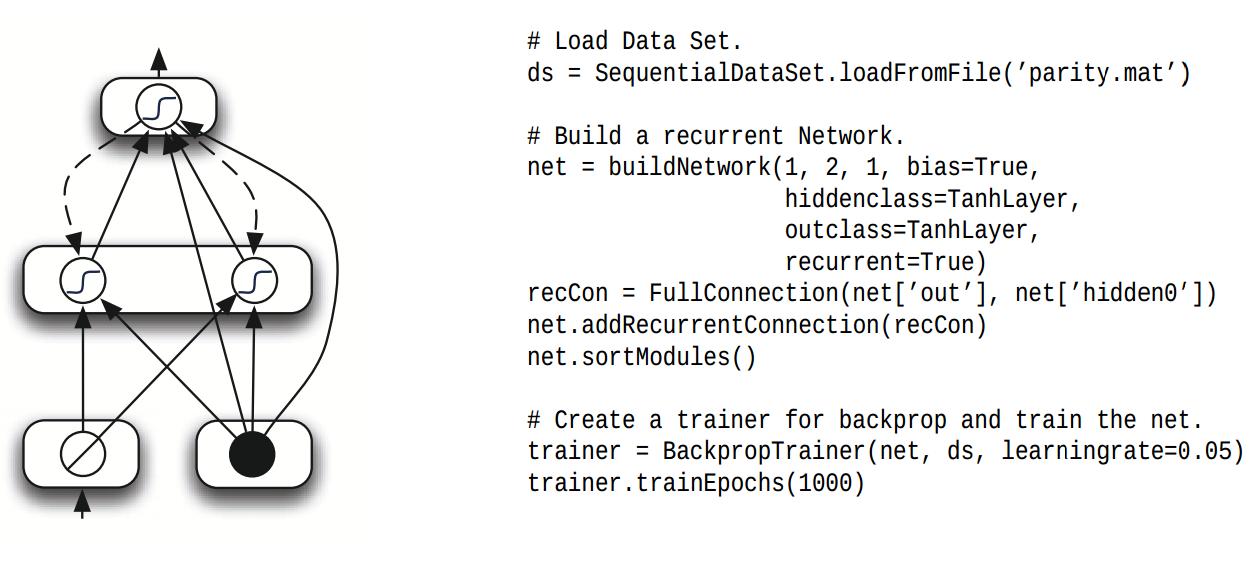
\includegraphics[width=0.8\textwidth]{nnet.png}%
    \caption{Example for a Basic Neural Network. Source: \cite{pybrain2010jmlr}}
    \label{fig:nnet}%
\end{figure}

\cite{pybrain2010jmlr} shows in figure~\ref{fig:nnet} a solution for the sieve problem. As Python is an interpreted language, 
speed bottlenecks can occur. Pybrain has a part of its underlaying functions rewritten in C-Code with bindings to Python.

One very important feature of Pybrain is the training module. The \texttt{dataset} object has a wide array of options to avoid programming
with Pythonic arrays. Concretely, it means going through multiple fields of input or expected output value with an iteration. 

Pybrain offers some visualisation wrappers around Pylab but the output is limited so the author used his own direct Pylab access.

\section{Pygame}

Pygame is a framework for game development in Python. It is focused on 2D development but not limited as bindings in OpenGL
exist. Pygame itself uses the graphical output wrapper SDL, the Simple DirectMedia Layer. Through this abstraction the 
operating system's native hardware accelerated libraries can be used.

Professional and commercially available games are programmed with Pygame as for example the graphical storytelling game
``Dangerous High School Girls In Trouble'' from~\url{http://www.mousechief.com/dhsg/index.html}.

The technical layout design is oriented to a graphic primitive object called \texttt{surface}. It can be used for displaying text
or loading images from file sources. Rotating, movement and collision detection is included in the methods. Most instantiation 
is handled through inherited classes. Initializing the main screen in windowed or full screen mode sets the whole resolution pixel 
numerated into a surface called \texttt{pygame.display}.
Next major best practice due to the online documentation from~\cite{pynew} is how to refresh the screen. As Pygame does 
not use 3D acceleration of graphical extension hardware except indistinctly specified. It comes at a cost of stability and
can disable inter-platform operability by not being able to run on Linux platforms.
As a general rule of thumb only the modified image or textual \texttt{surface} objects should be repainted each frame. The
practical problem comes with the layer laying in the back, i.e. the background in the last case. It will get painted black
as in leaving a trail.

Concluding the change of other \texttt{surface} objects a \texttt{display.flip()} repaints the background and tries to use
hardware to speed up the process if available. For a smooth feeling for fluid movement perception one second of animation
requires at lest 25 images. Therefore, a clock is running in the background is created which limits the output of frames 
per second with the \texttt{clock.tick(25)}.

Making the surfaces, redrawing them if needed and repainting the background can be put into one permanent \texttt{while:} structure.
This could already be a very basic but running game.

One additional topic for beginners not covered extensively on-line at~\cite{pynew} is the control interface. There are 
basic object for mouse click and movement events but also joysticks are supported. Due to the object oriented structure
key press events were not fully recognized when pressed simultaneously or in very short succession.


\chapter{Implementation}
\label{chap:impl}

After learning how to use the underlaying frameworks and accessing the brainwave scanner the game was programmed as a glue for all these 
components. It is the practical hands-on project work on the two weeks programme.

Most following work will use the explained frameworks in the previous chapter. The detailed explanation of the brain interface programming is 
in~\cite{pm} as this part will concentrate on the game. 


\begin{lstlisting}[language=Python,caption=Initialisation]
import pygame, math, random, thread
from pygame.locals import *

pygame.init()

screenwidth = 800
screenheight = 600
\end{lstlisting}

Game relevant functions and objects are stored in the \textit{game.py} file. The above code shows it is loosely bound, not using 
includes from the other objects like the brain interface or neural network. It was done to keep the file runnable without the special
hardware for debugging purpose. Second line is for a direct name for the modules in \texttt{pygame.locals} as constant names for key press names.
Screen size was adapted to fir on a small external screen like a projector. Automatic detection for full screen is possible but can be 
a hindrance while programming as threads may fail thus leaving the whole application frozen.


\begin{lstlisting}[float,language=Python,caption=Player Sprite Module, label=psprite]
class Sprite(pygame.sprite.Sprite):
    def __init__(self):
        self.image = pygame.image.load("zombie.png").convert_alpha()
        self.rect = self.image.get_rect()

        self.reset_position()
        self.speed = 3 

        self.normal_friction = .95 
        self.slowing_friction = .8

        self.target = None 
\end{lstlisting}

The player's in-game avatar is kept in a module as his properties are very different from other game objects as shown in listing~\ref{psprite}. He is a graphics primitive from a 
PNG picture which has its transparent alpha channels converted to fit into the background. It is an extension to the previous chapter \texttt{convert()} 
in Pygame as the transparency is stored in a new dimension per pixel in addition to the three colors. Setting it to values around 100 could create a 
half-transparent look.
Friction is saved as an constant for the moving methods of the player's avatar. Targets get calculated when both movement vectors are set, i.e. horizontal
and the initial speed.


\begin{lstlisting}[float,language=Python,caption=Player's Avatar Movement,label=movement]
    def update(self):
        
        self.dir = self.get_direction(self.target)
        if self.dir:
            
            if self.distance_check(self.dist):
                self.speedX += (self.dir[0] * (self.speed / 2))
                self.speedY += (self.dir[1] * (self.speed / 2))
                self.speedX *= self.slowing_friction
                self.speedY *= self.slowing_friction
            else:
            [..]
\end{lstlisting}

In listing~\ref{movement} shown method is the player's avatar \texttt{update()} to recalculate the new position of the sprite and repaint it. Only the 
first half of the method is shown which checks if a movement action was issued by the player. The conditional statement checks if 
the traveled distance is above the estimated target position and if so slows the player's avatar down. The numerically higher 
friction value is applied. Not shown is the equivalent code for normal movement and the drawing itself.  

\begin{lstlisting}[float,language=Python,caption=Group of Targets,label=group]
class BrainSpriteCollection():
    def __init__(self):
        self.brainSpriteList = pygame.sprite.RenderPlain()
    def reset(self):
        self.brainSpriteList.empty()
        for i in range(7):
            brainSprite = BrainSprite()
            brainSprite.rect.x = random.randrange(screenwidth)
            brainSprite.rect.y = random.randrange(screenheight - 200)
            self.brainSpriteList.add(brainSprite)
    def returnList(self):
        return self.brainSpriteList
\end{lstlisting}

A single \texttt{BrainSprite} is put together in a group of 7 other sprites. They are stored in a list of sprites for 
easier collision detection and resetting as visible in listing~\ref{group}. If the player's avatar hit one or more of the brain sprites an event is 
called which removes the visible brain sprite from the game and add one point to the hit counter.
Noteworthy to show the random initialisation of the single brain sprite's position. It never spawn at the bottom line of the
screen to avoid strange player movement towards the opposite of the player's avatar viewing direction.
The version of this source code excerpt for the brainwave scanner adds improved random numbers collected from the
brain action of the player. Whether such numbers are numerically more random is explained in more detail in~\cite{pm}.

The logically following source code of variable initialisation is skipped as it contains no especially interesting detail.


\begin{lstlisting}[float,language=Python,caption=Start of Main Loop,label=mloop]
clock = pygame.time.Clock()
running = True

while running:
    clock.tick(30)
    for event in pygame.event.get():
        if event.type == pygame.QUIT:
            running = False
\end{lstlisting}

Main loop as described in the framework chapter about Pygame is displayed in the code of listing~\ref{mloop}. \texttt{running} is 
a boolean variable for the determination of ending or continuing the loop. It is checked against at the top so 
clicking on the window closing button or typing the operating systems own cancelling key press will abort the main loop thus
the application after a cleanup.  
More events are processed after the visible code excerpt like for events from the brainwave scanner or manual keyboard usage.
The clock is set at 30 frames per second to give a smooth running perception to the player's eye.

\begin{lstlisting}[float,language=Python,caption=Collison Detection,label=coll]
hitlist = pygame.sprite.spritecollide(sprite, brainSpriteCollection.returnList(), True)
        if len(hitlist) > 0:
                score +=len(hitlist)
                scoreTextSurfaceObj = fontObj.render('Total Score: ' + str(score), True, (0,0,0), (155,0,0))
                print "hit"
                thread.start_new_thread(plopSound.play,())
\end{lstlisting}

Last point of the shown code of the main game is the collision detection in listing~\ref{coll}. At first, the 
amount of hit sprites in one frame are queried. Through the first method's \texttt{spritecollide()} parameters 
the player's avatar is set in at first, following the group of collectable brain sprites and finally a \texttt{true} for
removing a brain sprite of the visible and drawable list of targets. 
The score is updated on each additional hit in a custom font in a special \texttt{surface}. It is also painted in red for 
better visibility on the back and white background.
A sound for acoustic notification of a scoring hit is played in a thread to not let the main thread wait for it finishing playing.

Omitted source code of the game are the painting\footnote{Called blitting in Pygame's documentation} method calls and some minor 
actions. 

Another important part was the development of the neural network. Some code examples will be shown for the most interesting parts.

The dozen import lines are not shown as the majority are alias calls to shorten the length of following module names. A module for
reading and writing CSV\footnote{Comma Separated Files} is used for saving the training results of neural networks when adjusted for 
a player. Graph creating modules from the Pylab framework are utilised for creating statistical comparison data between 
runs of the recording session, i.e. one game run.

\begin{lstlisting}[float,language=Python,caption=Design of the Neural Network, label=nnet]
self.neuralNet = FeedForwardNetwork()
        inLayer = LinearLayer(7)
        hiddenLayer = SigmoidLayer(5)
        outLayer = LinearLayer(1)

        self.neuralNet.addInputModule(inLayer)
        self.neuralNet.addModule(hiddenLayer)
        self.neuralNet.addOutputModule(outLayer)

        self.neuralNet.addConnection(FullConnection(inLayer,hiddenLayer))
        self.neuralNet.addConnection(FullConnection(hiddenLayer,outLayer))

        self.neuralNet.sortModules()
\end{lstlisting}

The code in~\ref{nnet} shows the code of the complete neural network. It is composed of seven input gates for the seven slices of the FFT 
value from the brainwave scan. The input layer is fully connected to the hidden layer, i.e. every gate is connected to every gate in 
a higher layer. The result is the single output gate. This setup was acquired through testing where a higher amount of hidden layer 
stations resulted in lower speed and less amount in an unusable output value.  

\begin{lstlisting}[float,language=Python,caption=Training of the Neural Network, label=ntrain]
if self.trainMode:
    ds = self.makeTrainingSet(savedData)
    trainer = BackpropTrainer(self.neuralNet,ds,verbose=True)
    trainer.trainUntilConvergence(maxEpochs=10)
    self.printGraph(ds)
    NetworkWriter.writeToFile(self.neuralNet, "lastNetwork.xml")
\end{lstlisting}

Listing~\ref{ntrain} shows the method calls for running backpropagation algorithms on the created neural network. Basically, it adjusts the threshold
value of every gate according to a simulated training function which is seeded with mean values from a training session. The training session takes
ten second and calculates a mean value for standardized brain wave ranges. These ranges indicate if a user is more or less mentally excited in a
time frame. The \texttt{printGraph()} call is a reference to the lengthly image diagram object. The network and its connection weights and threshold values
are saved with the network layout in a XML file. The file will be used for further training and is improving the ranges through every subsequent run.

Not shown code of the practical part include the drawing functions, the loading and saving functions in CSV files and the parameter division for startup
options. 


\begin{lstlisting}[float,language=Python,caption=Generating Training Values, label=ngen]
    def makeTrainingSet(self,savedData):
        ds = SupervisedDataSet(7,1)
        meanValue = self.getMeanValue(savedData)
        correctionFactor = 0
        for line in savedData:
            correctionFactor += (line[0] - meanValue[0]) * 3
            correctionFactor += (line[1] - meanValue[1]) * 2
            correctionFactor += (line[2] - meanValue[2])
            correctionFactor += (meanValue[3] - line[3])
            correctionFactor += (meanValue[4] - line[4]) * 2
            correctionFactor += (meanValue[5] - line[5]) * 3
            correctionFactor += (meanValue[6] - line[6]) * 6
            ds.addSample(line,correctionFactor)
            correctionFactor = 0
        return ds
\end{lstlisting}

In listing~\ref{ngen} the generation of training values are shown in code. A dataset is instantiated where the mean values of the previous runs 
are fetched from another method. Their slices difference is a numerical value from the mean values and the current status including a changing factor.
Lower indices of the arrays correlate with the frequency range starting from 2 Herz which are signs for slow spiking human neurons. Fast spiking neurons
indicate mental activity but are generated with smaller amplitude. Concluding, a meditating or mentally engaged 
player can get very visible action compared to a normal mind state.



\chapter{Evaluation}
\label{chap:eva}

calibration time
learning algorithms

\chapter{Summary}
\label{chap:sum}

\nocite{*}
\bibliographystyle{acm}
\bibliography{common}
\listoffigures
\lstlistoflistings

\end{document} 
